\begin{figure}[h!]
    \centering
    \caption{Changes in Chicago-Naperville-Elgin CBSA due to a counterfactual raise 
    	     of the federal MW to \$9 in January 2020}
    \label{fig:map_chicago_cf_wkp_res}
    
    \begin{subfigure}{.49\textwidth}
        \caption*{Changes in residence MW}
        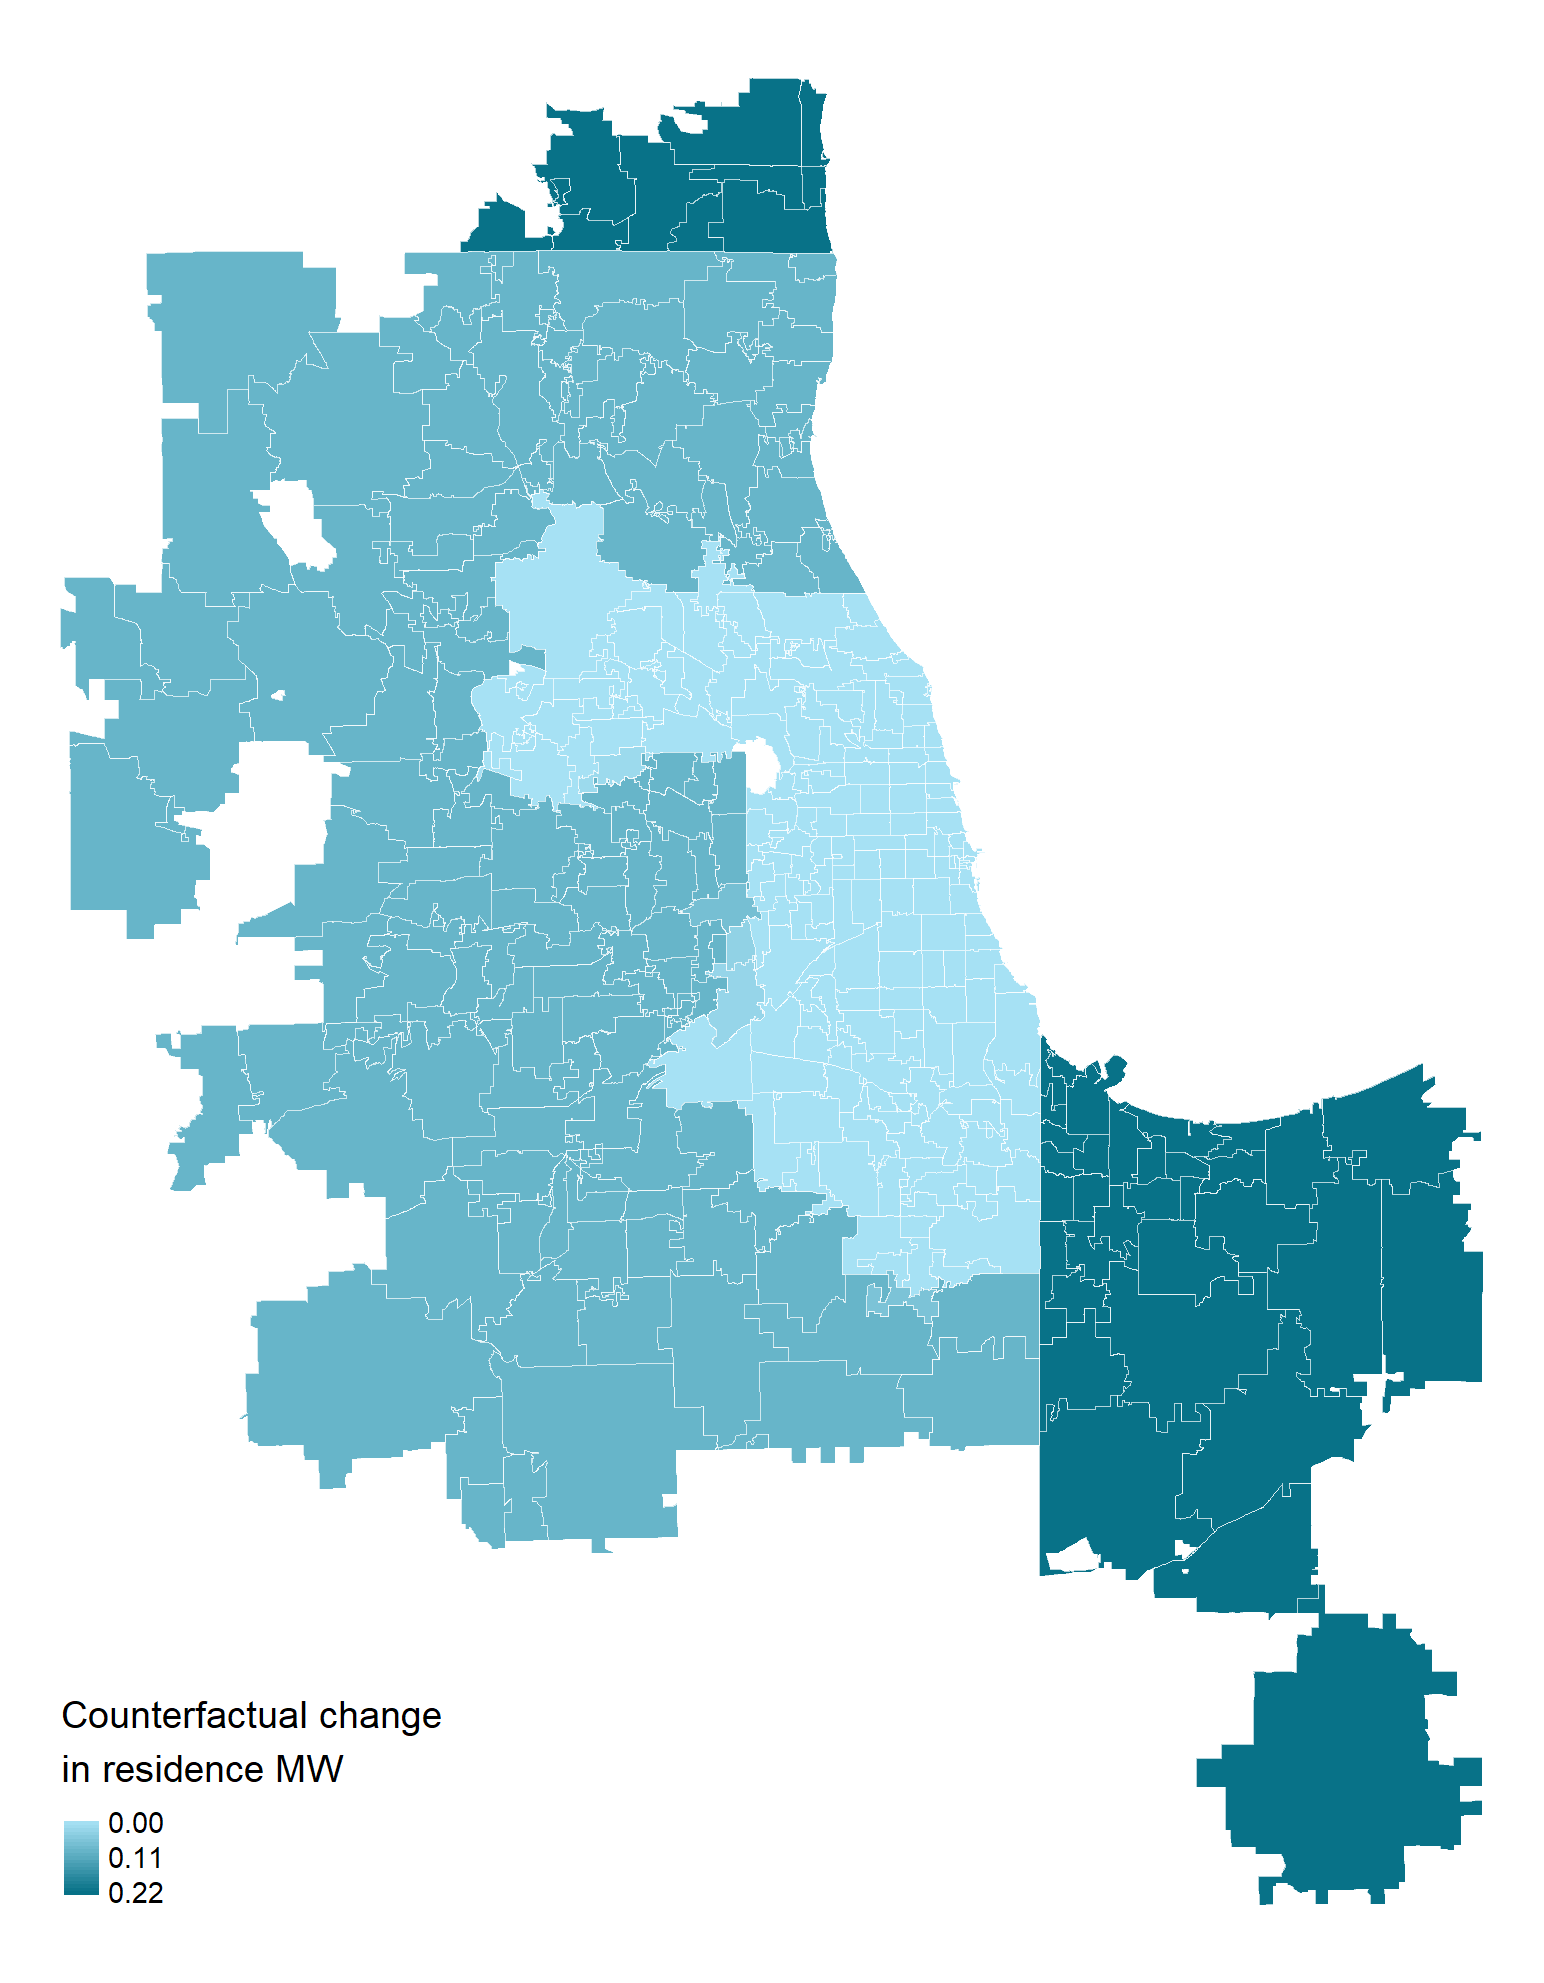
\includegraphics[width = 1\textwidth]
            {counterfactuals/output/chicago_d_mw_res.png}
    \end{subfigure}%
    \begin{subfigure}{.49\textwidth}
        \caption*{Changes in workplace MW}
        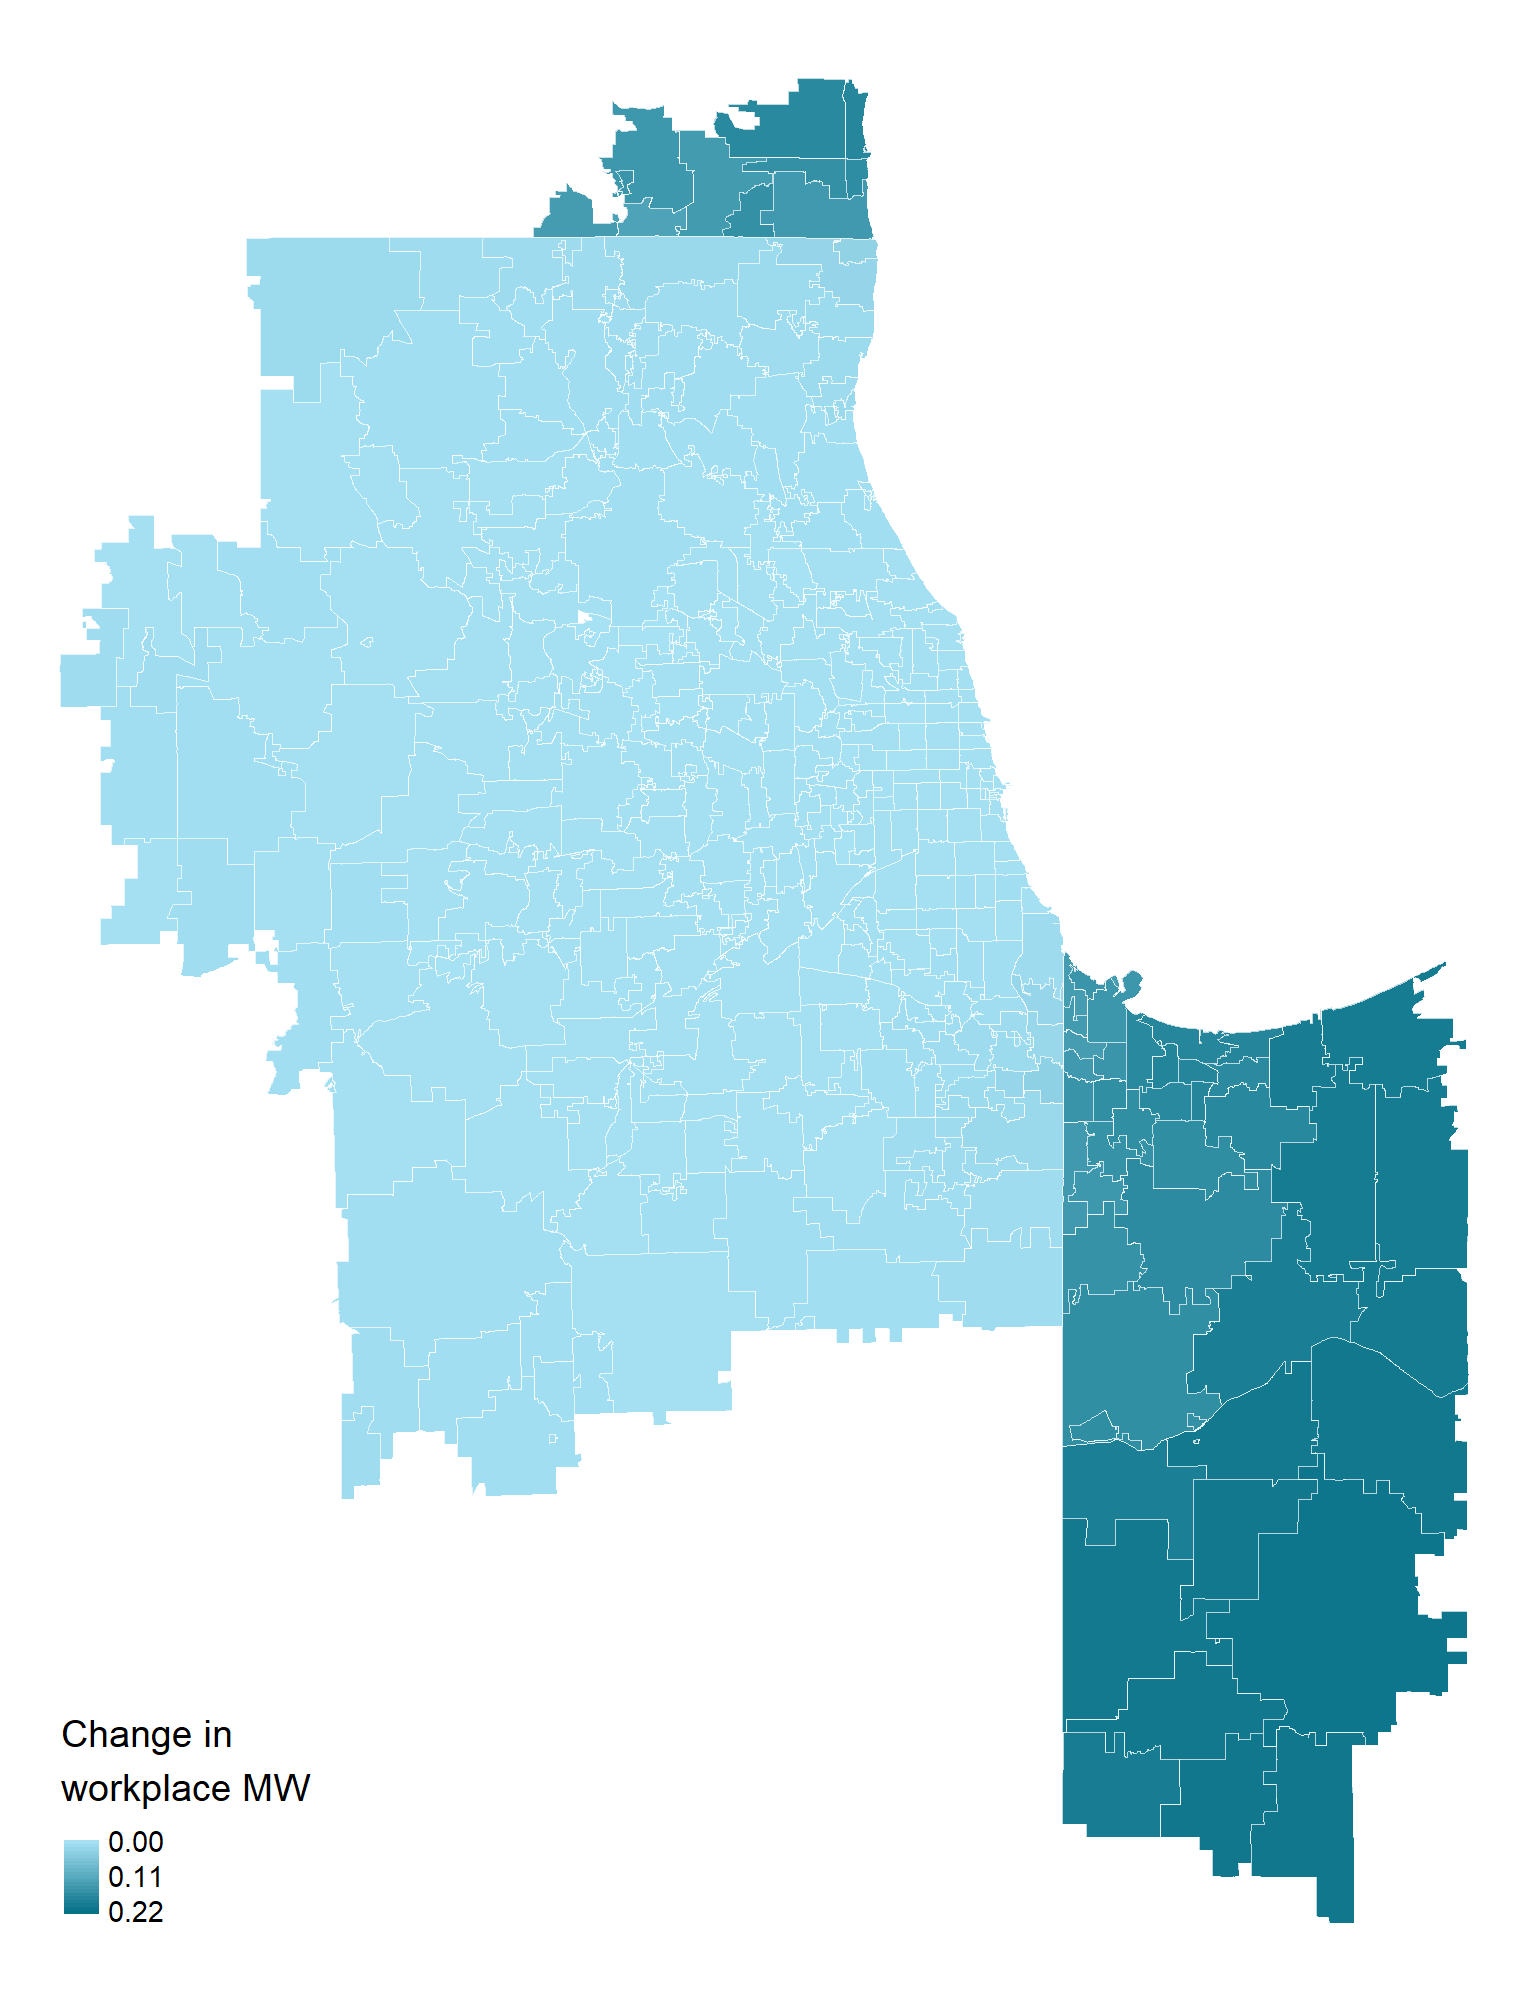
\includegraphics[width = 1\textwidth]
            {counterfactuals/output/chicago_d_mw_wkp.png}
    \end{subfigure}

    \begin{minipage}{.95\textwidth} \footnotesize
        \vspace{3mm}
        Notes: 
        Data are from LODES and the minimum wage panel described in Section 
        \ref{sec:mw_construction}.
        The figures maps changes in the residence and workplace MW measures 
        generated by a counterfactual increase to \$9 in the federal MW in 
        January 2020, holding constant other MW policies in their December 2019 
        levels.
    \end{minipage}
\end{figure}
